\subsection{Sequence Diagram}

\begin{figure}[h!]
\centering
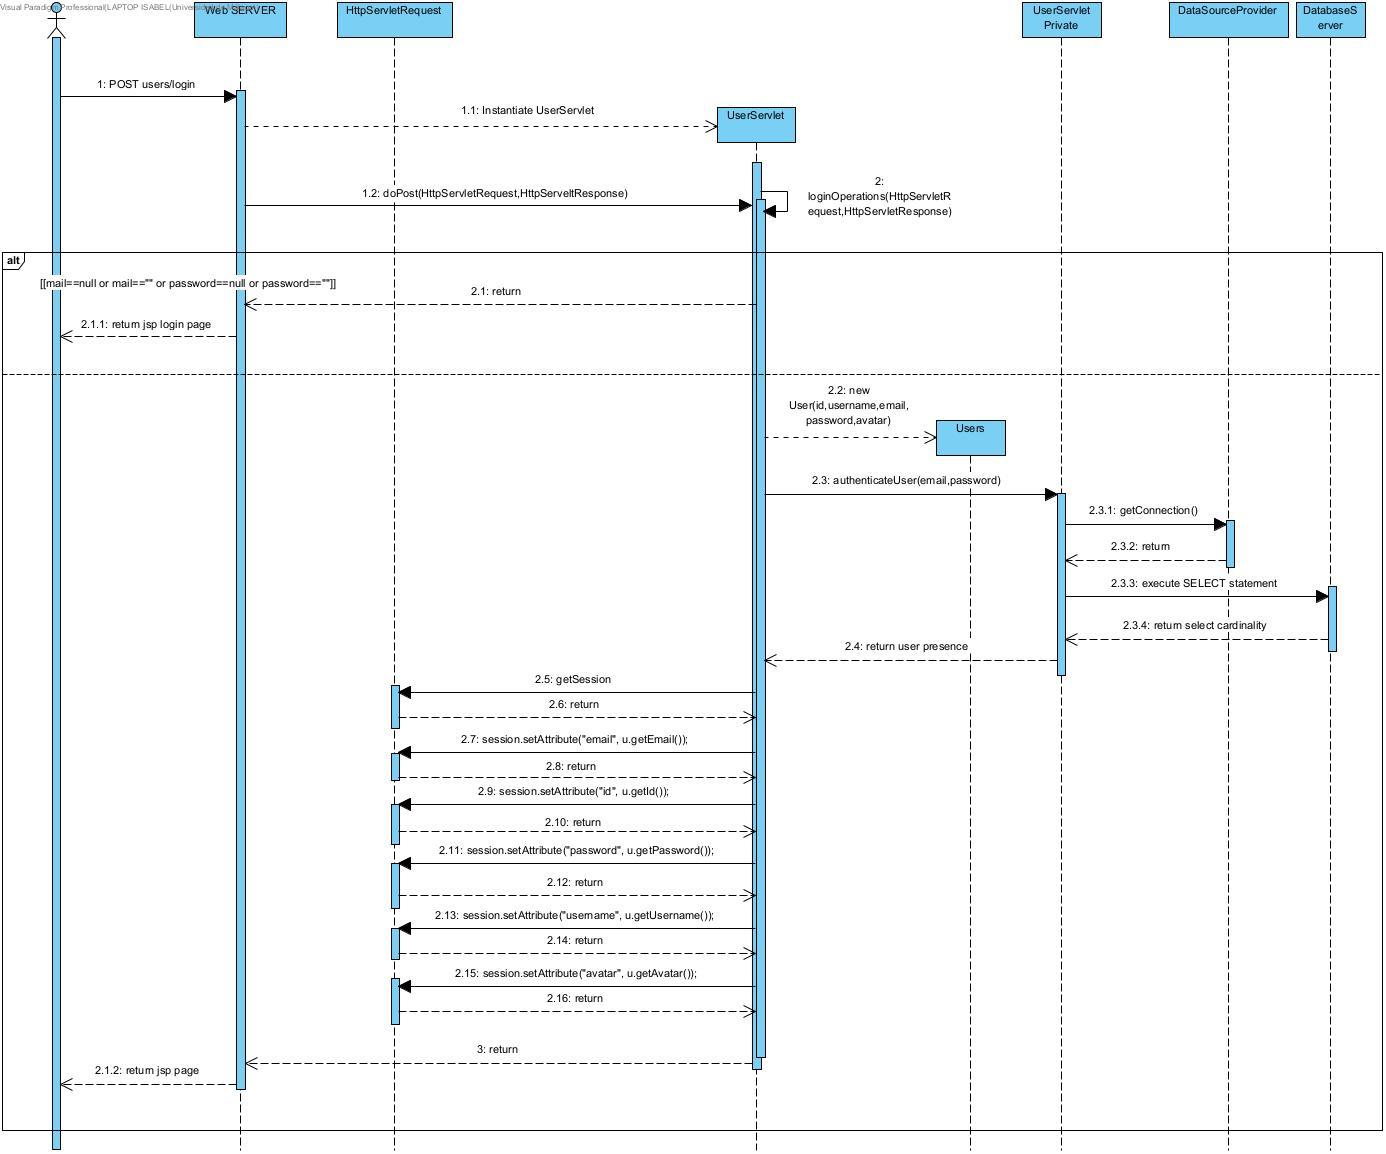
\includegraphics[width=0.9\textwidth]{sections/BLL/Sequence Diagram.jpg}
\caption{Class Diagram}
\end{figure}

%describe here the sequence diagram

Here reported the sequence diagram for the login. The user executes a POST request to the Web Server with the URI users/login. The data about the user that is trying to make the login (email and password) are passed to the web server. The web server initiates the UserServlet and calls the method doPost passing the attributes needed. The UserServlet analyzes the request and recognise it as a login operation, then it calls the method loginOperations. This method controls whether the email and password have been correctly provided, using the private method authentificateUser (that has a connection with the DataSourceProvider) that access the database, if the data is correct, returns the login.jsp page, if not it shows a error. Else, a new user is initialized with the data. The method authentificateUser checks if in the database is a user with the email and password provided. After that, the control is returned to the UserServlet, which obtains the session for the HttpServletRequest and sets five parameters in the session, which are the attributes of the user.
